\documentclass[fontsize=12pt]{article}
\oddsidemargin=-1cm
\textwidth=18cm
\textheight=20cm
\setlength{\parindent}{10mm}
\setlength{\parskip}{0.9em}
\def\baselinestretch{1.5}

\usepackage[spanish]{babel}
\renewcommand {\spanishtablename}{Tabla}
\usepackage[utf8]{inputenc}
\usepackage{graphicx}
\usepackage{caption} 
\usepackage{amsmath, amsthm, amsfonts}
\usepackage{enumerate} 
\usepackage{fancyhdr}
\usepackage{anysize} 
\usepackage[usenames]{color}
\usepackage{booktabs}

\pagestyle{fancy}

\chead{}
\lhead{} 
\rhead{}
\lfoot{\it }
\cfoot{}
\rfoot{\thepage}

\title{
\centering
Modelos Probabilistas Aplicados \\
Johanna Bolaños Zúñiga \\
Matricula: 1883900\\
Tarea 2
}

\date{}

\begin{document}
\maketitle

\section{Libro Seleccionado -- \textit{The Scarlet Letter}}

En el presente trabajo se realiza un análisis estadístico con datos  directamente desde la Web en el programa R versión 4.0.2 \cite{r}.

El análisis fue realizado con el libro \textit{The Scarlet Letter}, el cual se encuentra disponible de manera gratuita en \textit{Project Gutenberg} \cite{libro}.


\section{Análisis estadístico}
Para realizar el análisis estadístico y como ayuda visual se utilizaron diferentes tipos de gráficos. El código en R se encuentra en el repositorio de GitHub \cite{github}. 

Para llevar a cabo el estudio, se visualiza el libro tanto por la cantidad de \texttt{letras} como de \texttt{palabras} que hay en él.

En la Figura \ref{letras}, se muestran todos los caracteres Alfanuméricos utilizados en el libro. Sin embargo, nos interesan todos las letras, por lo cual, se procedió a realizar un filtro y, finalmente, obtenemos los datos mostrados en la Figura \ref{letrasfiltradas}, en la cual se puede observar todas las letras y la cantidad de veces en que fueron empleadas.


Para visualizar de una mejor manera la información anterior, se organizan de manera decreciente la frecuencia de las letras, ver Figura \ref{letrasfiltradasdecr}. También, se elabora un histograma con $3$ cubetas lineales, en la que podemos observar que son muy pocas las letras que tienen alta frecuencia de uso, ver Figura \ref{histograma}.


\begin{figure}
\centering
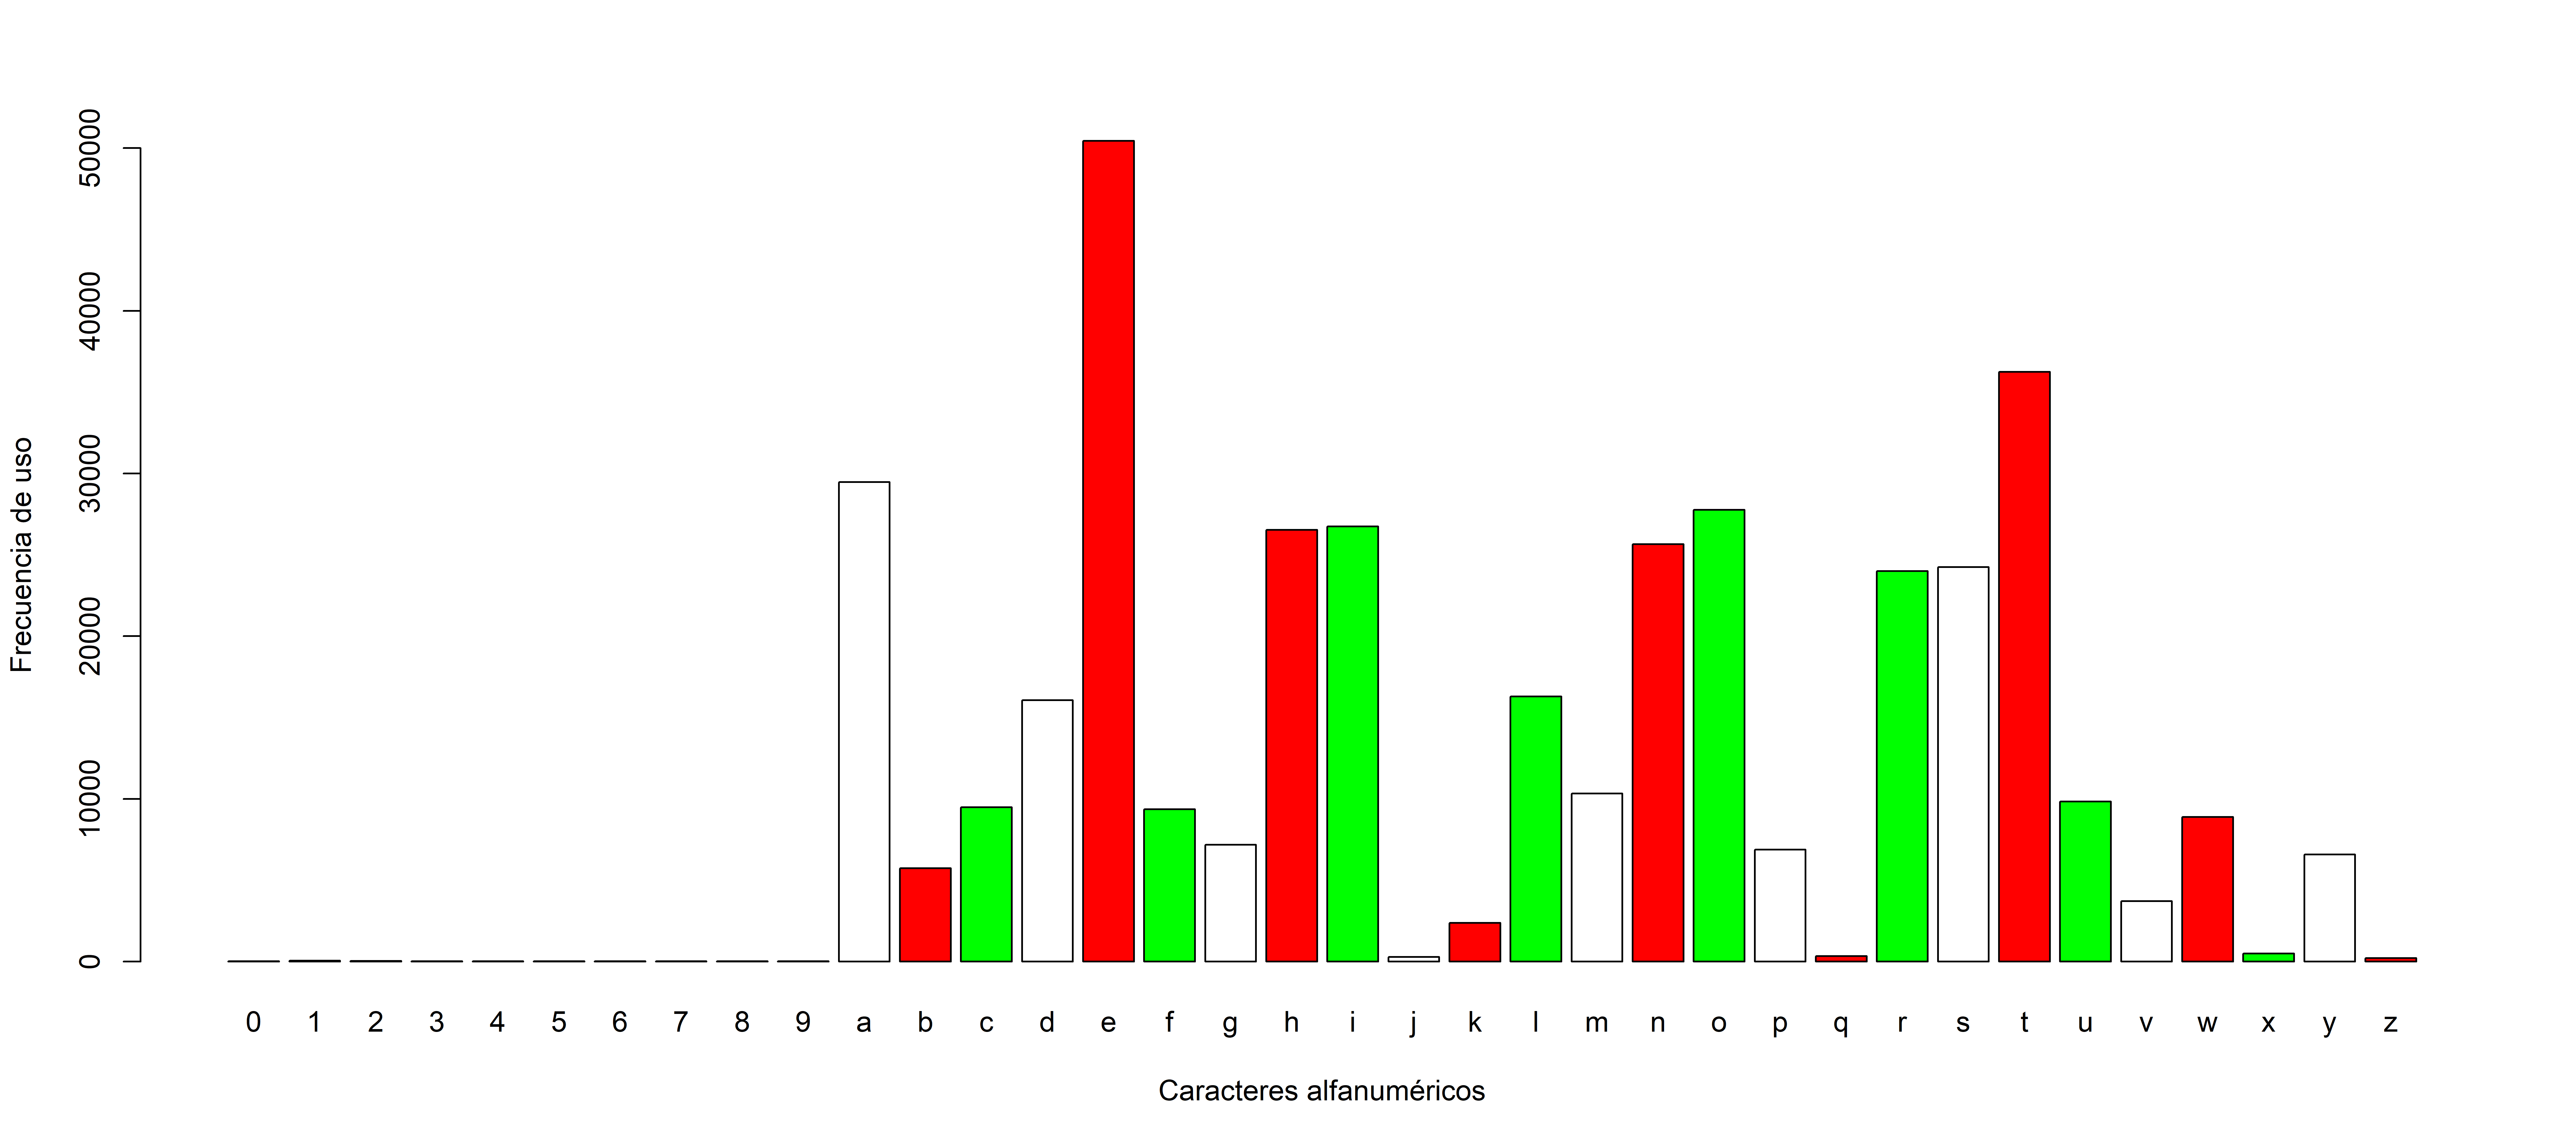
\includegraphics[scale=0.45]{Figures/letrasEnElTexto.png}
\caption{Frecuencia de los caracteres alfanuméricos del libro}
\label{letras}
\end{figure}


\begin{figure}
\centering
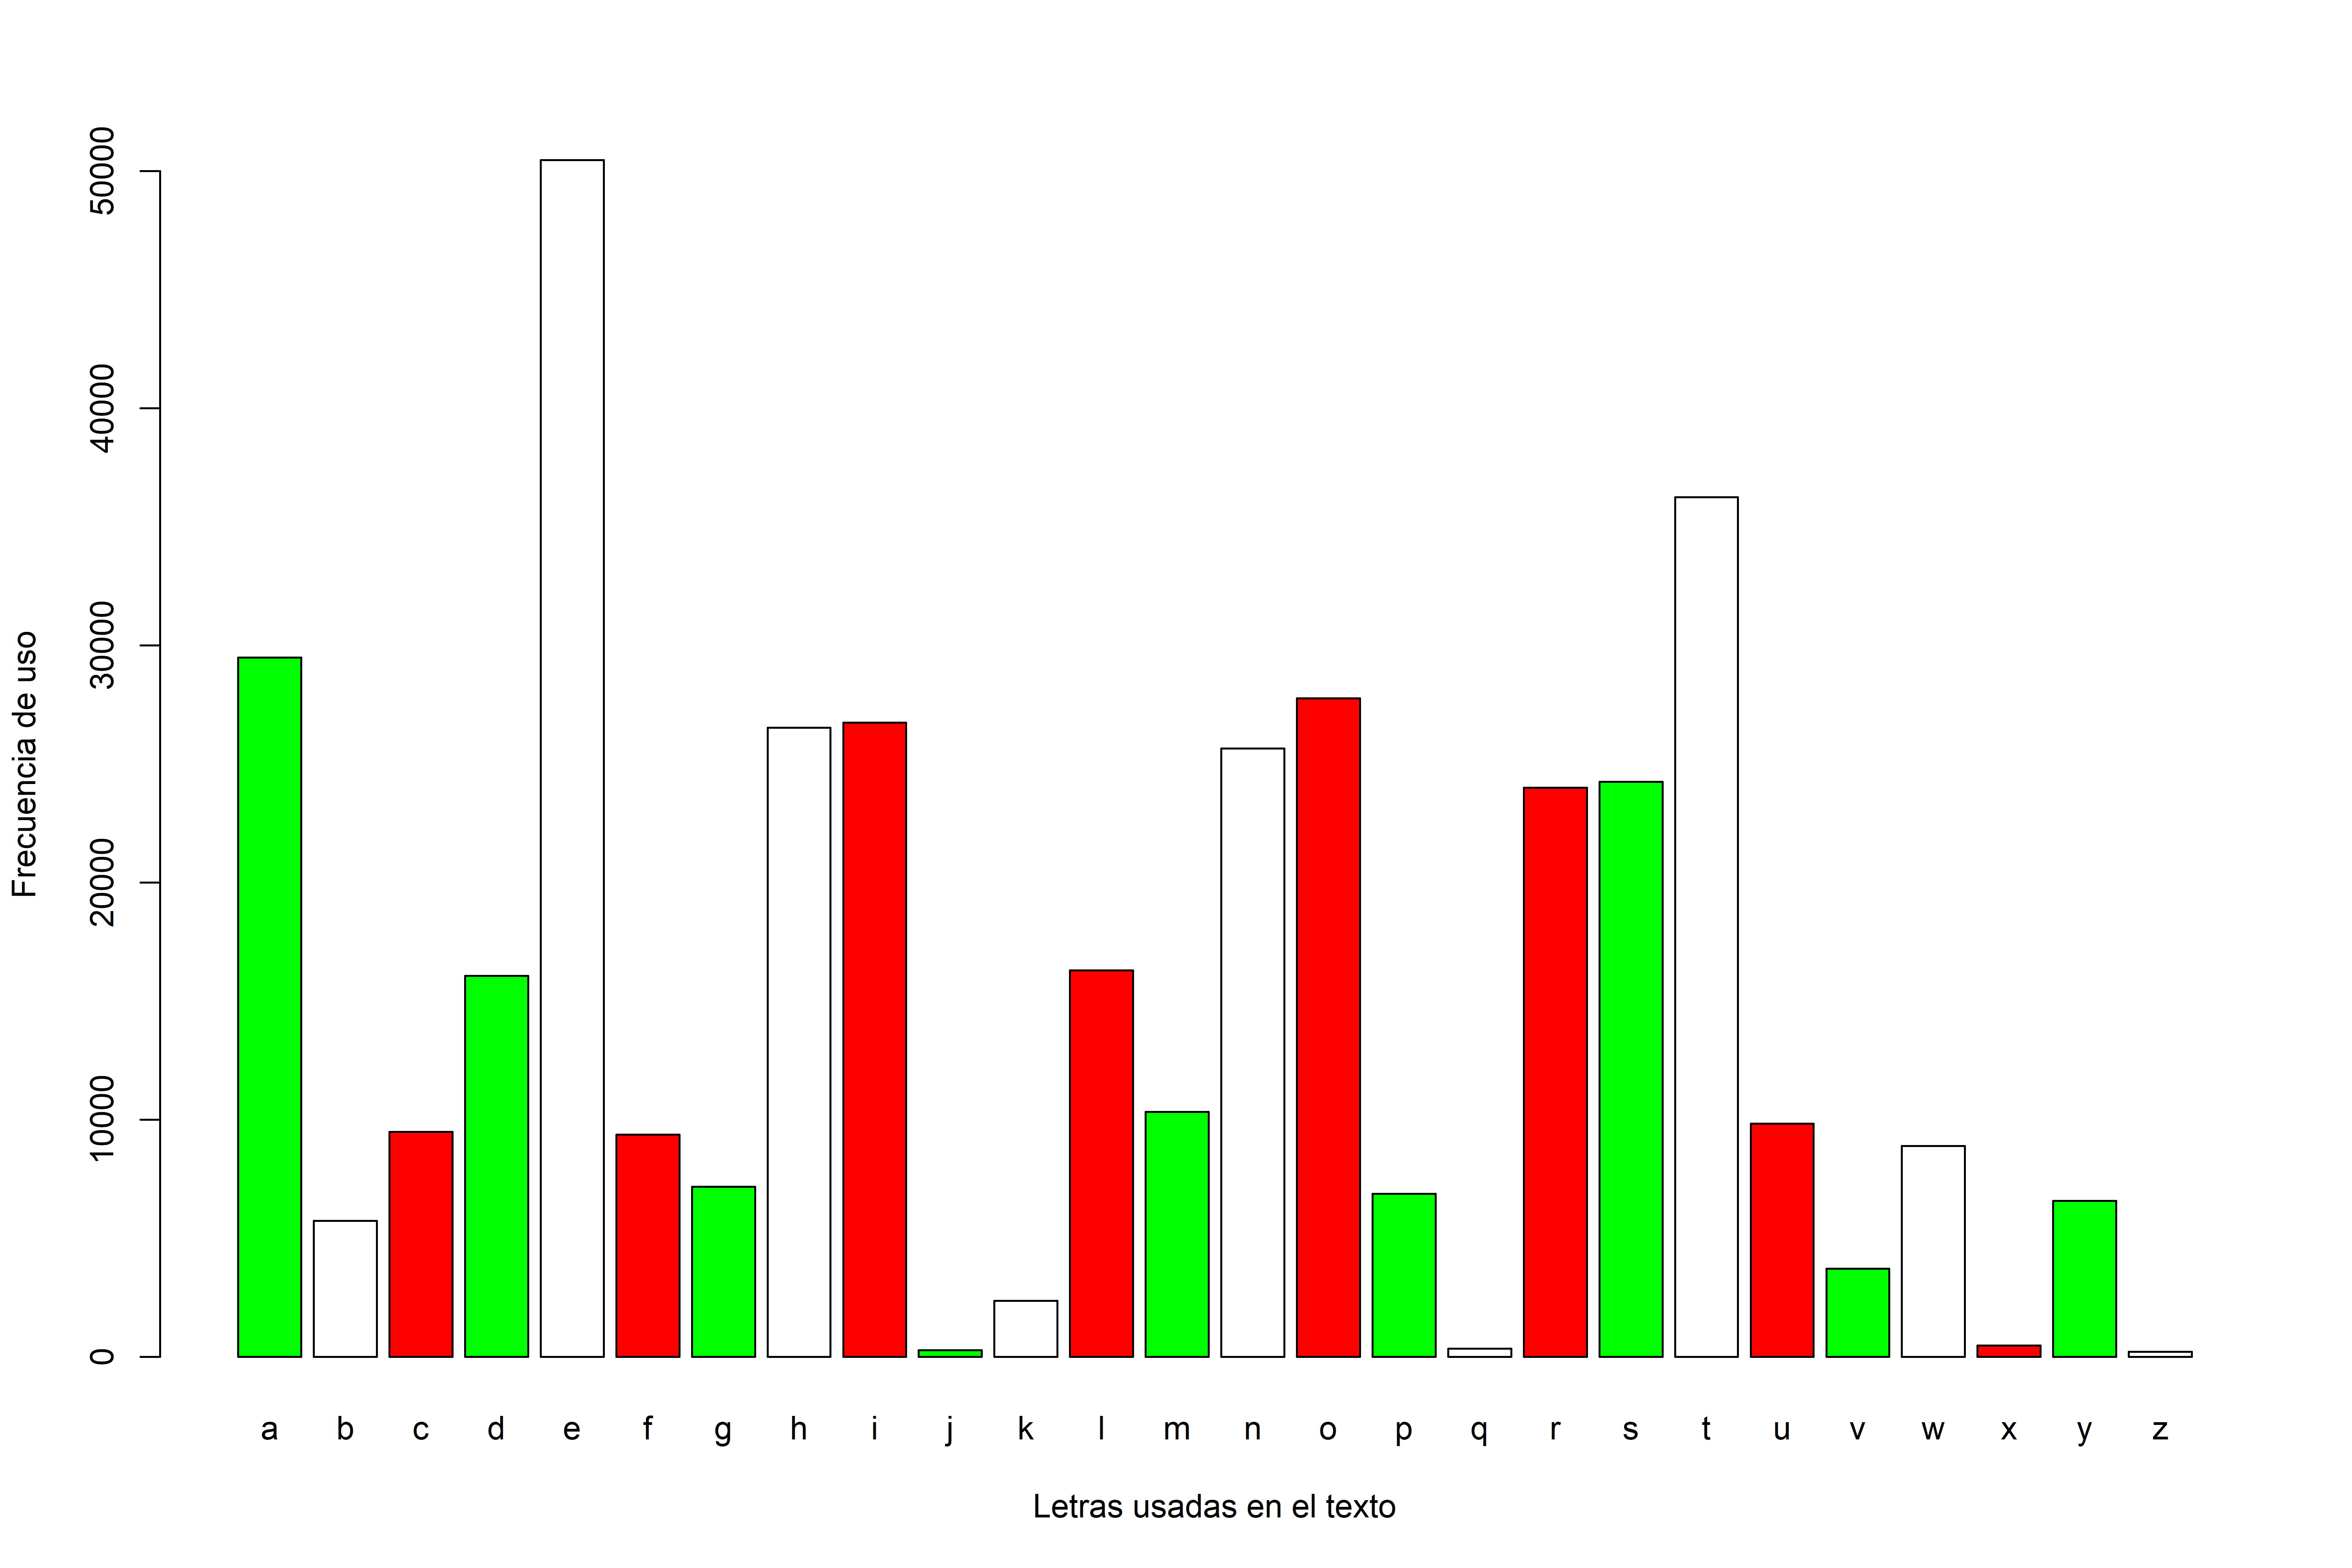
\includegraphics[scale=0.5]{Figures/letrasFiltradas.png}
\caption{Frecuencia de las letras usadas en el libro.}
\label{letrasfiltradas}
\end{figure}

\begin{figure}
\centering
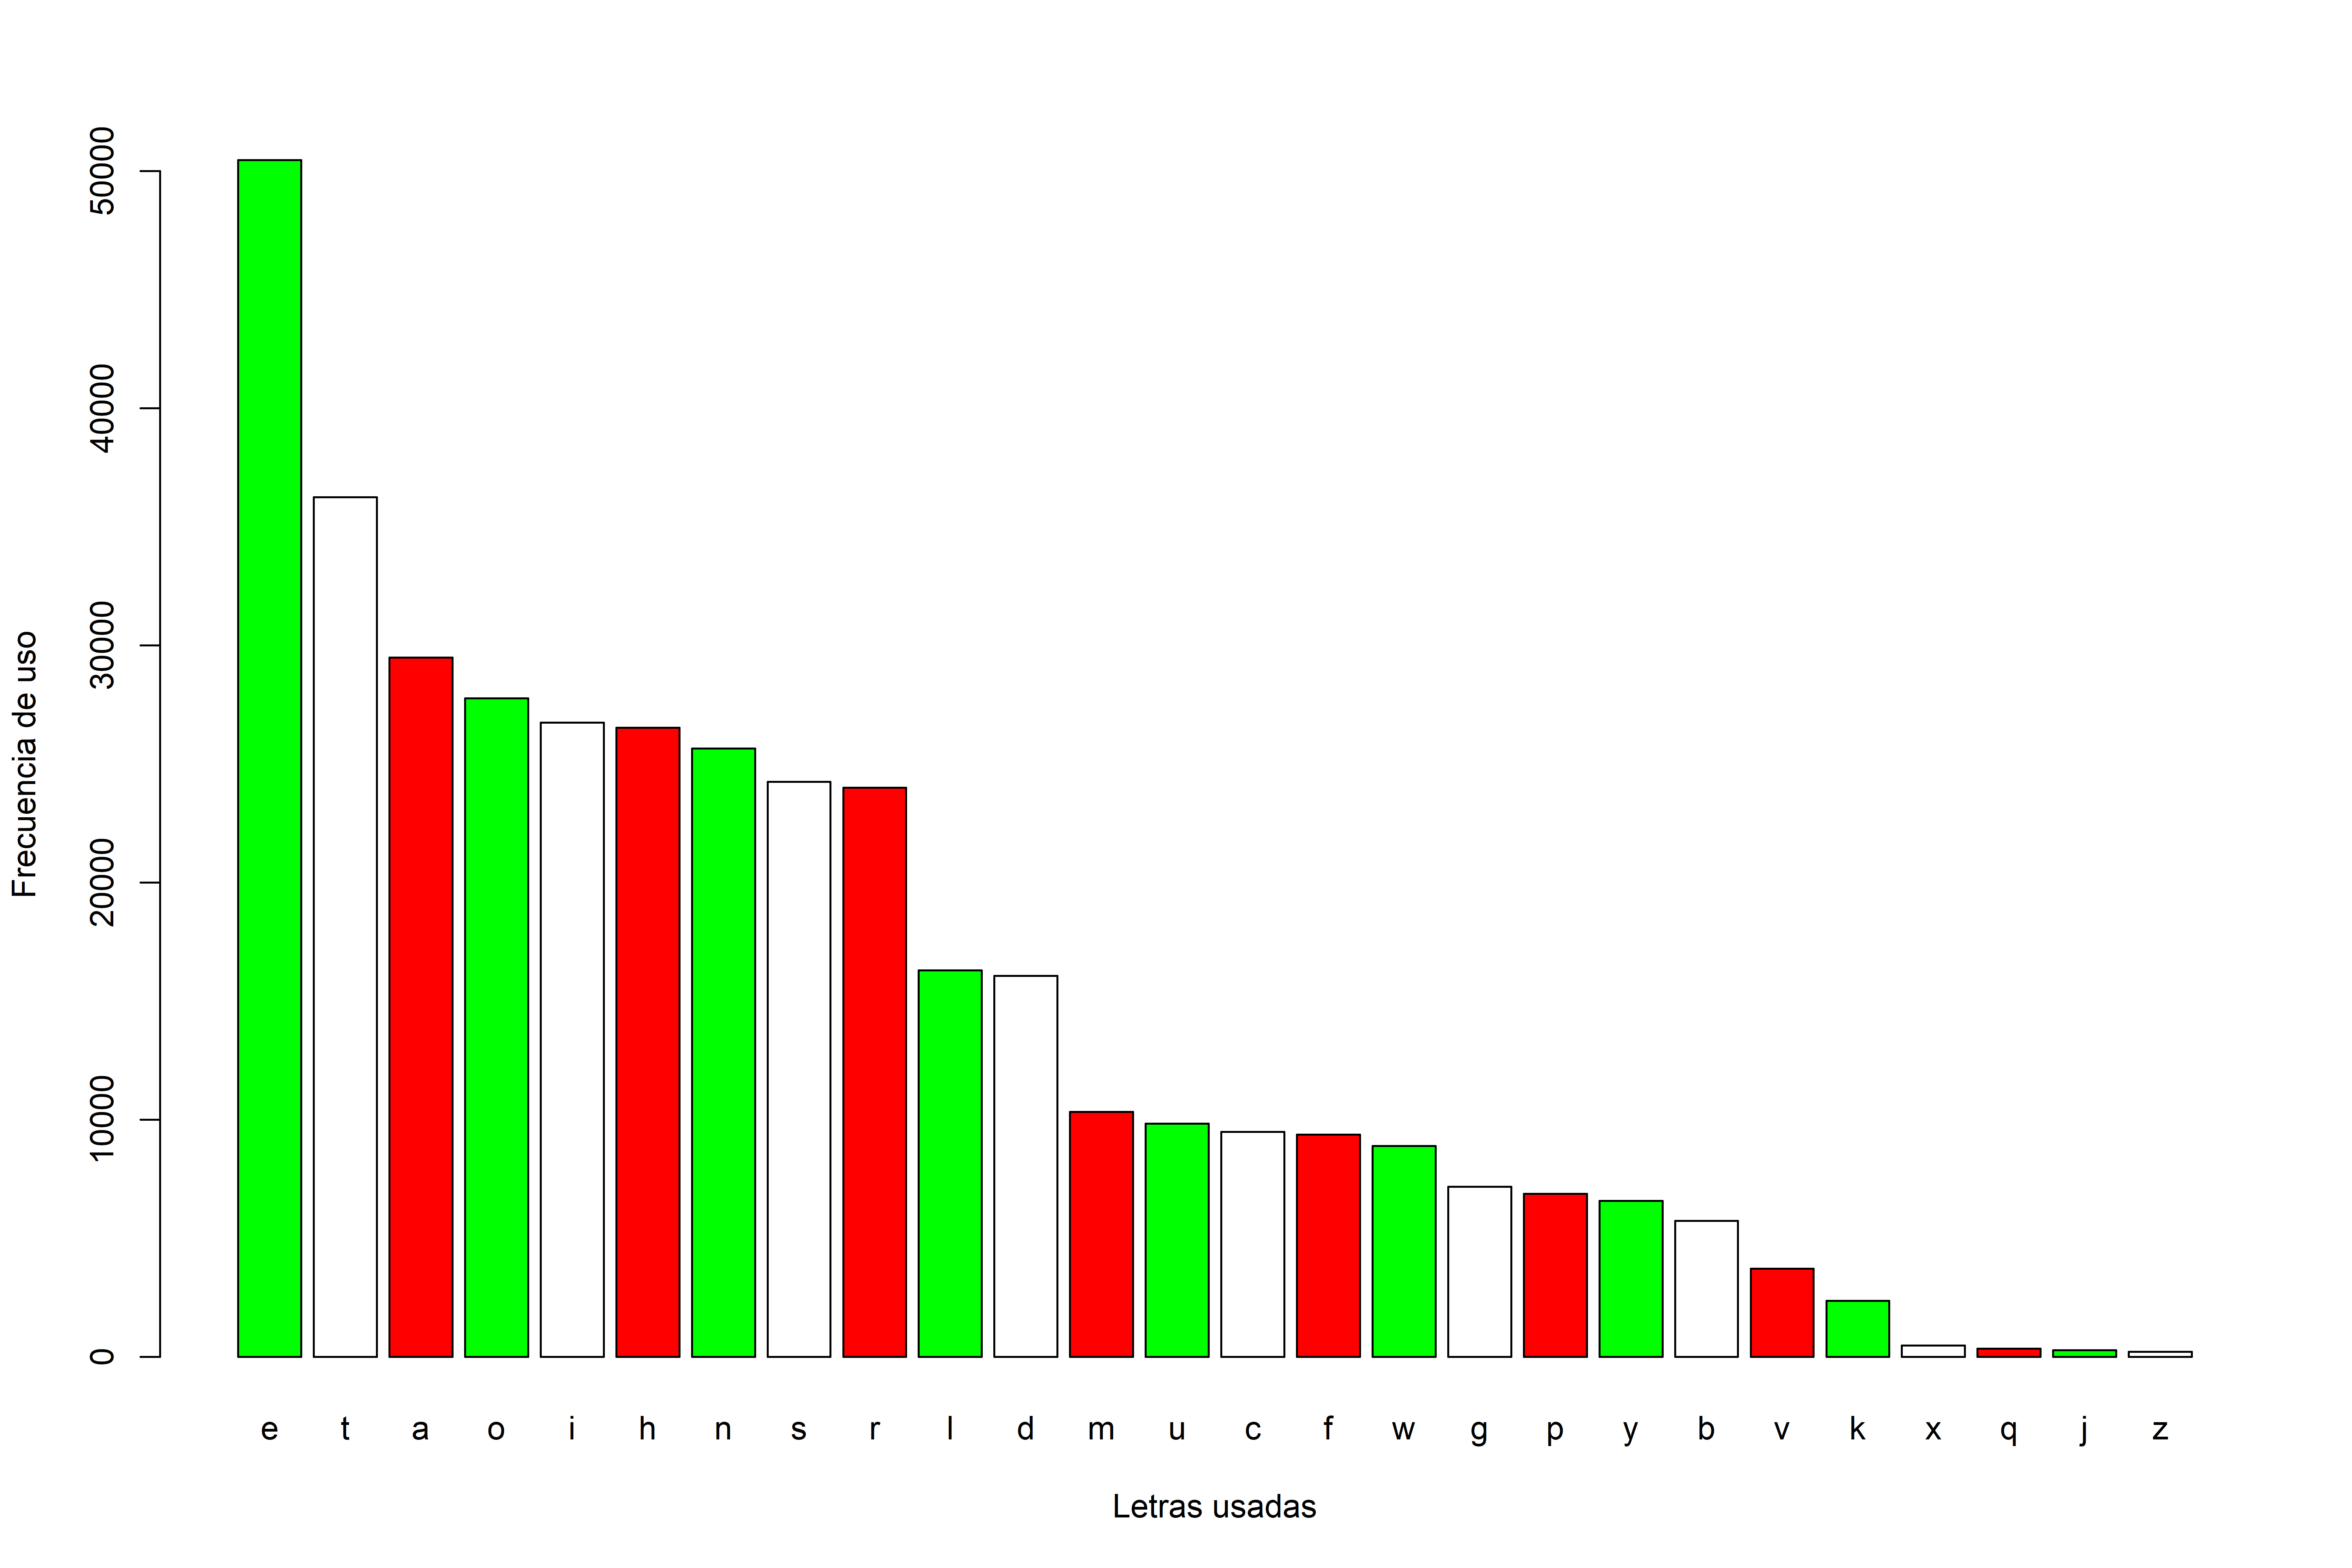
\includegraphics[scale=0.5]{Figures/letrasFiltradasDrec.png}
\caption{Frecuencia decreciente de las letras usadas en el libro.}
\label{letrasfiltradasdecr}
\end{figure}

\begin{figure}
\centering
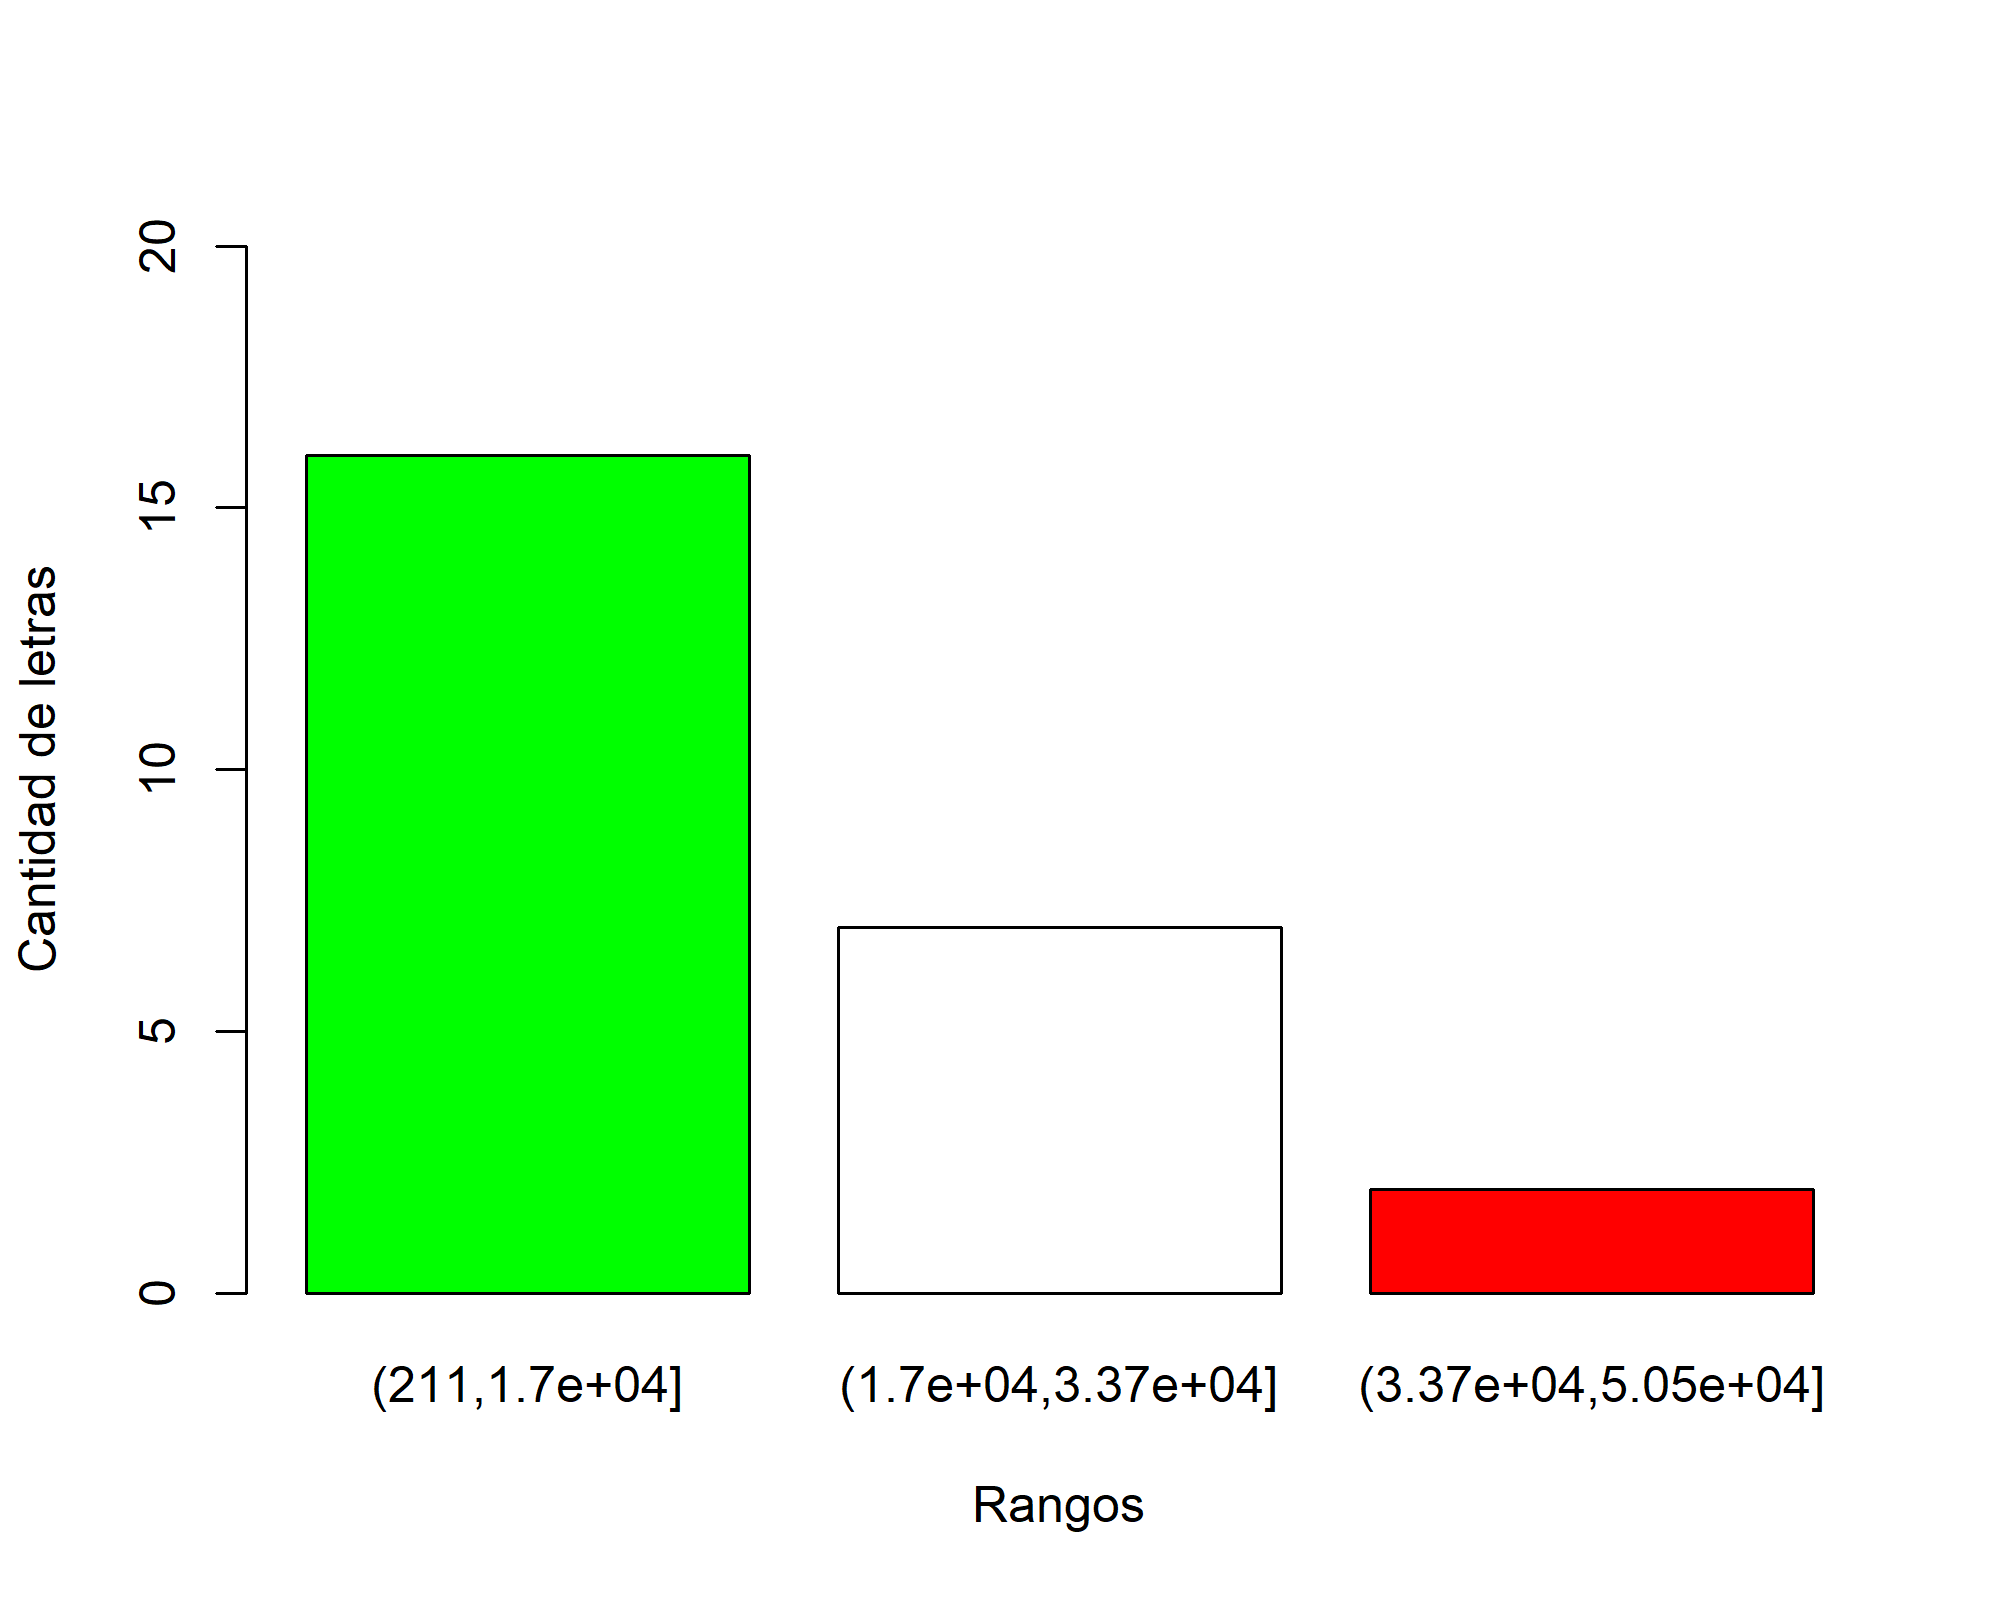
\includegraphics[scale=0.6]{Figures/histDeLetrasFiltradas.png}
\caption{Histograma de la cantidad de letras usadas en el libro.}
\label{histograma}
\end{figure}

En cuanto al análisis por \emph{palabras}, en la Figura \ref{palabras} se muestran todas las palabras usadas en el libro. Sin embargo, se puede observar que son tantas las palabras utilizadas que es difícil hacer una interpretación a partir de ella. Por lo anterior, se realizó una depuración de las palabras que aportan poca información, como son las preposiciones, artículos y conjunciones. Estas palabras son conocidas como \textit{stopwords}. 

En la Figura \ref{palabrasfiltradas}, se muestran las palabras que tienen una frecuencia superior a $150$. Para una mejor interpretación de los datos obtenidos, en la Figura \ref{palabrasfiltradasdec} se organizan de manera decreciente las palabras más usadas. 

De las palabras con mayor frecuencia podemos destacar que, la palabra más repetida es \texttt{Hester} y \texttt{Pearl}, lo cual tiene mucho sentido, ya que la primera es el nombre del personaje principal y la segunda, es el nombre de la hija. Sin embargo, a pesar de que \texttt{Prynne} es el apellido de la protagonista, el autor frecuenta más su nombre. En la Figura \ref{worldcloud} se muestra de una manera más didáctica las palabras más usadas en el libro, donde el tamaño es mayor para las palabras que aparecen con más frecuencia, este tipo de gráfica se conoce como \texttt{nube de palabras} o en inglés \textit{world cloud}.

\begin{figure}
\centering
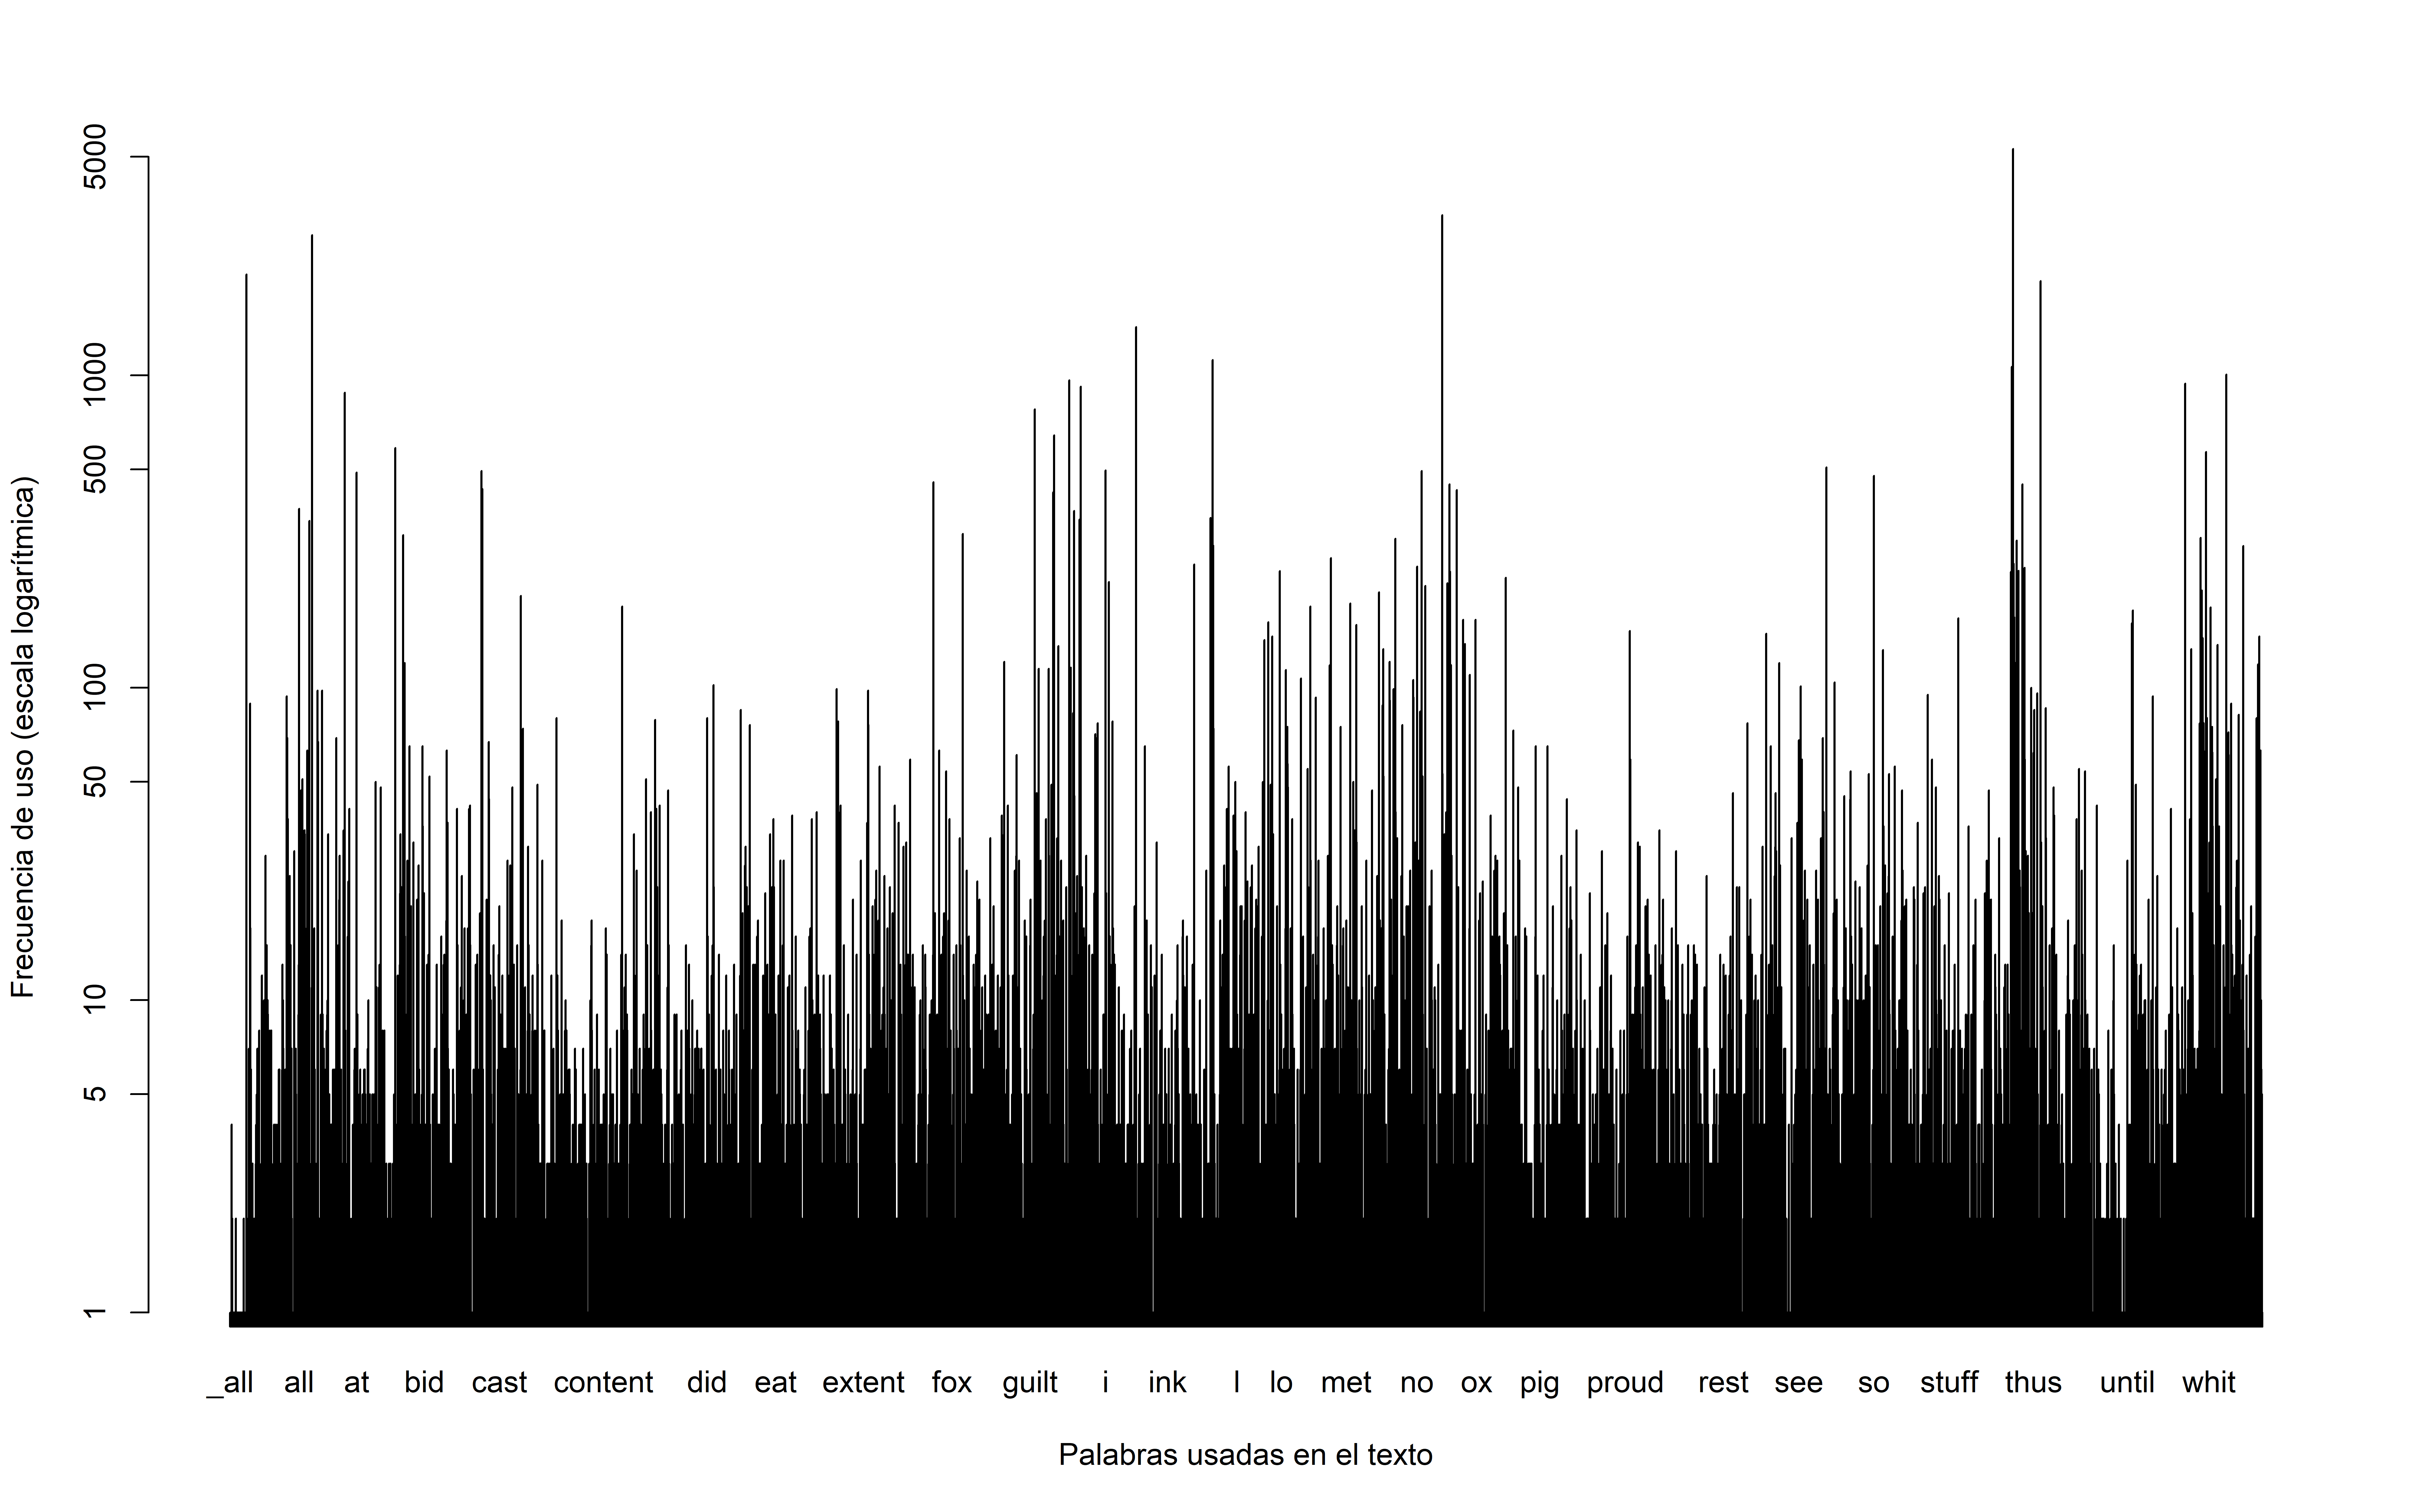
\includegraphics[scale=0.5]{Figures/palabrasEnElTexto.png}
\caption{Palabras utilizadas en el libro}
\label{palabras}
\end{figure}

\begin{figure}
\centering
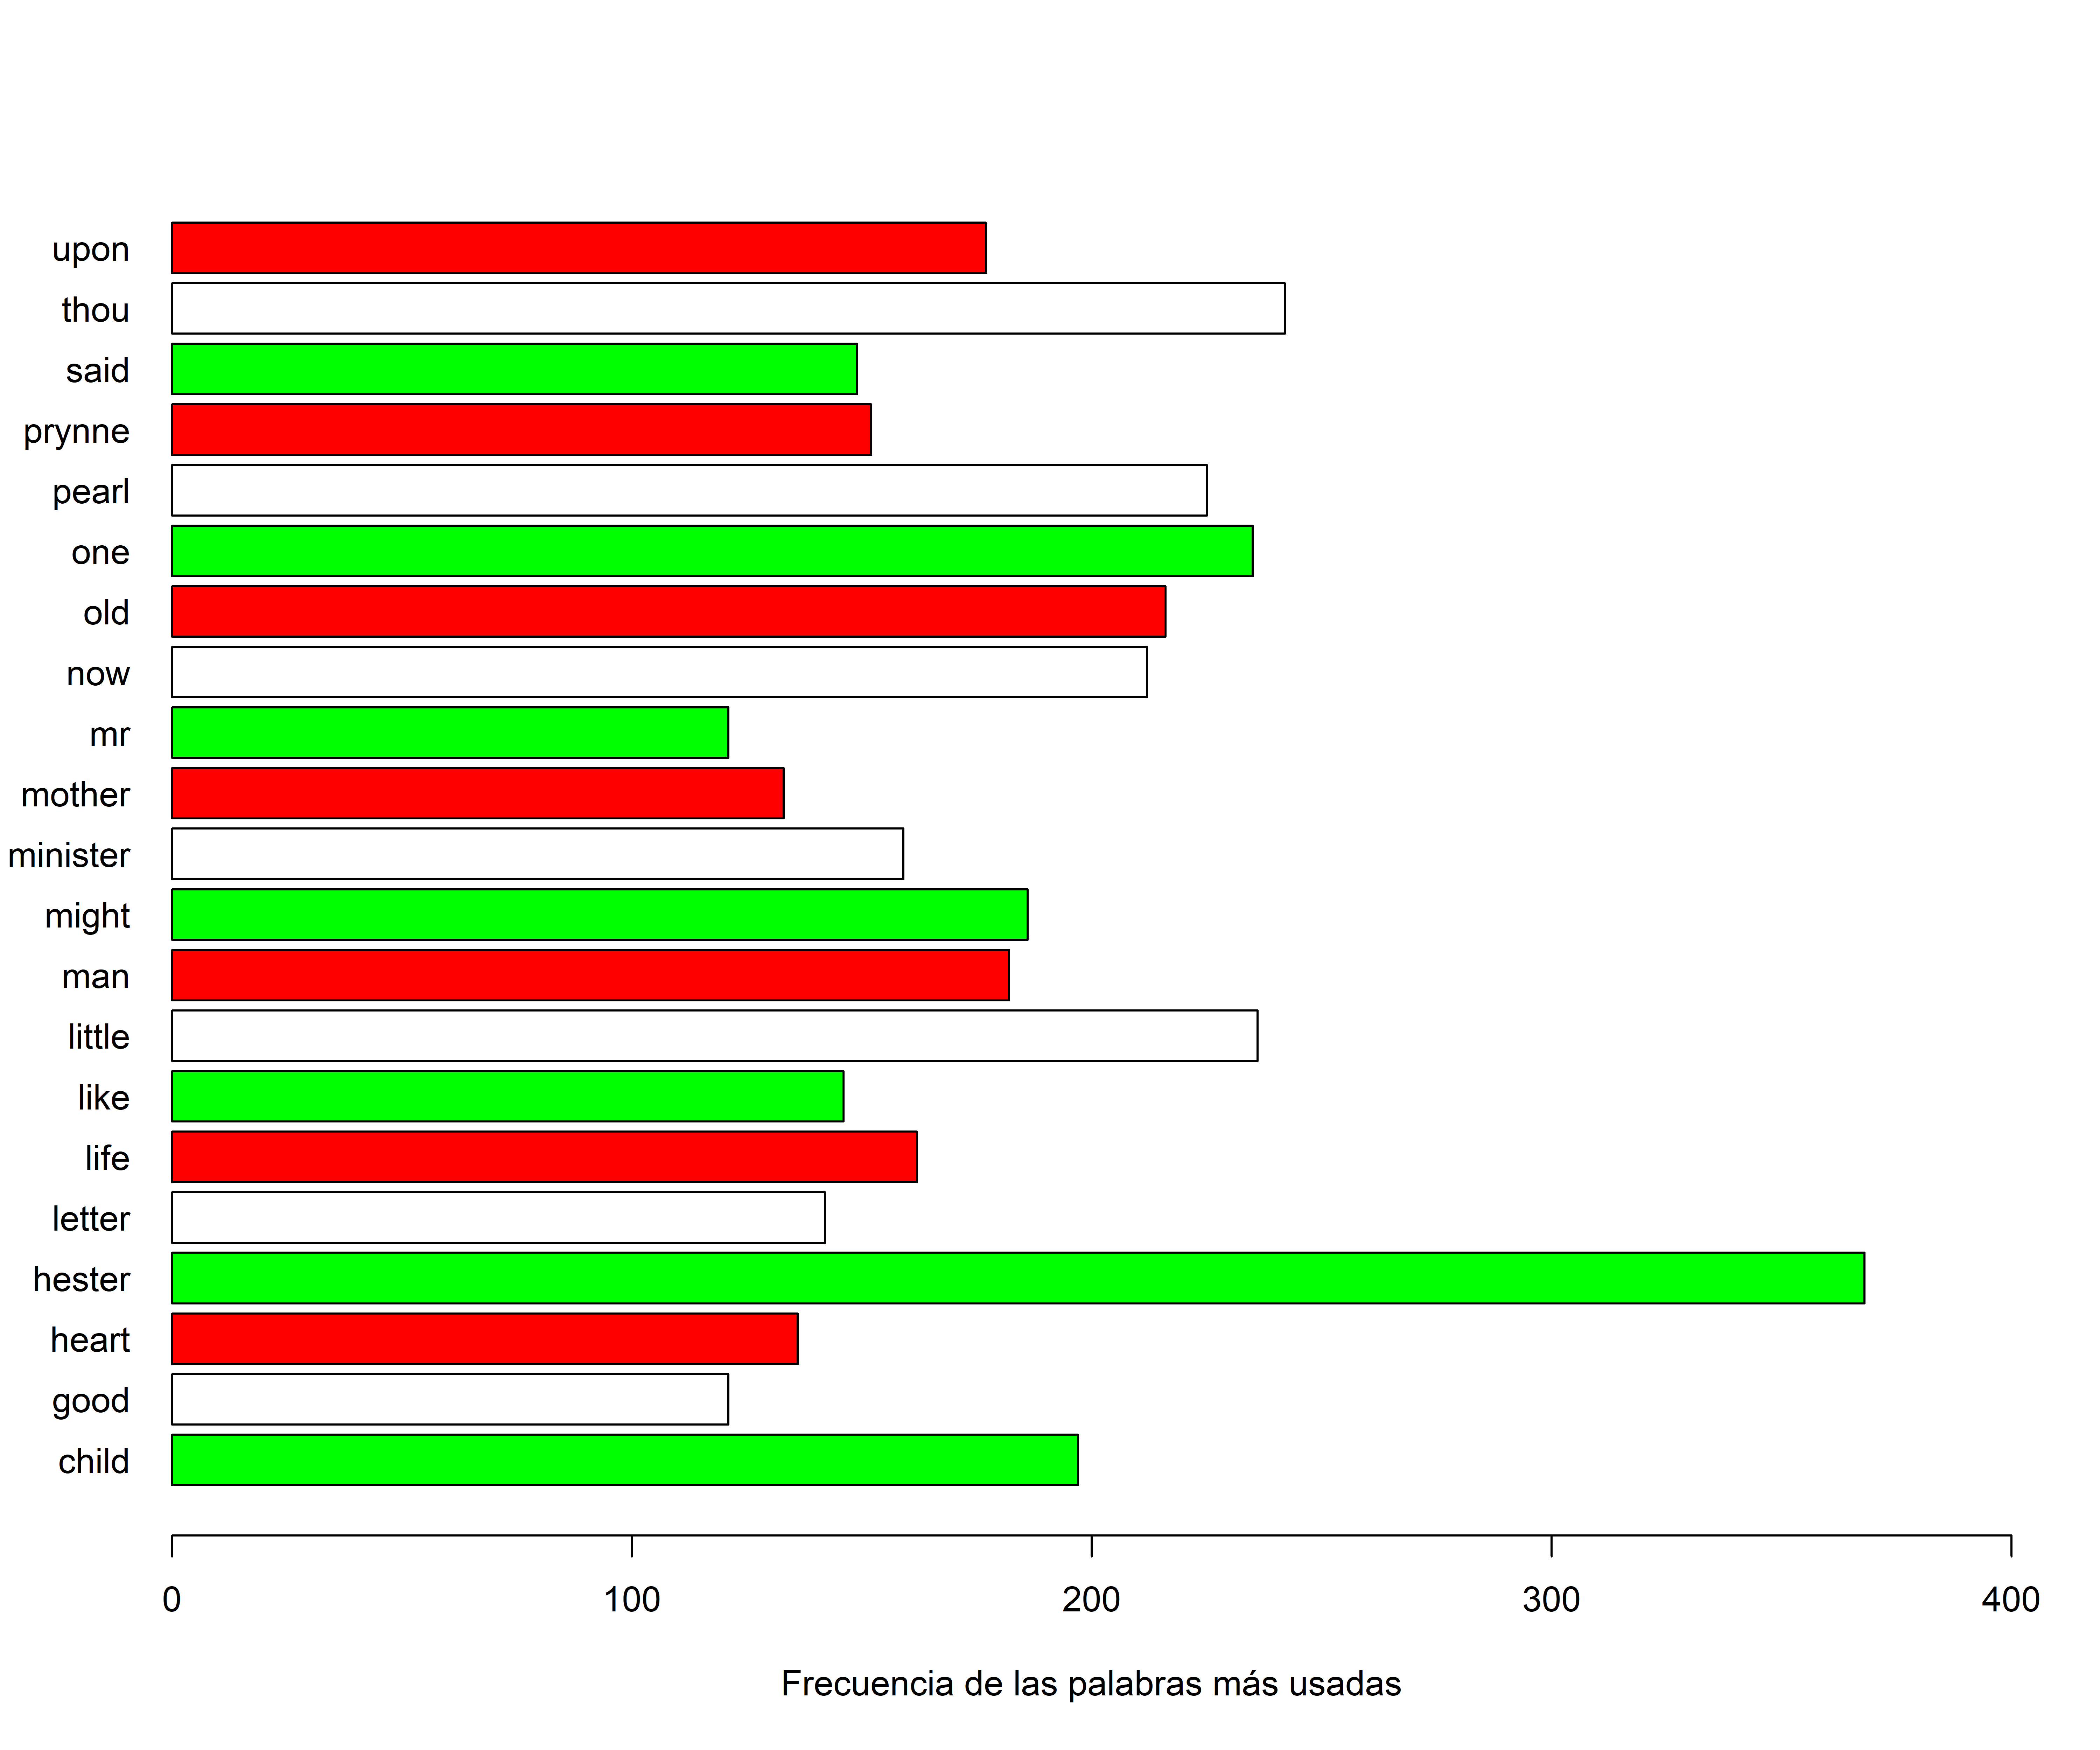
\includegraphics[scale=0.6]{Figures/palabrasFiltradas.png}
\caption{Palabras de mayor frecuencia en el libro}
\label{palabrasfiltradas}
\end{figure}

\begin{figure}
\centering
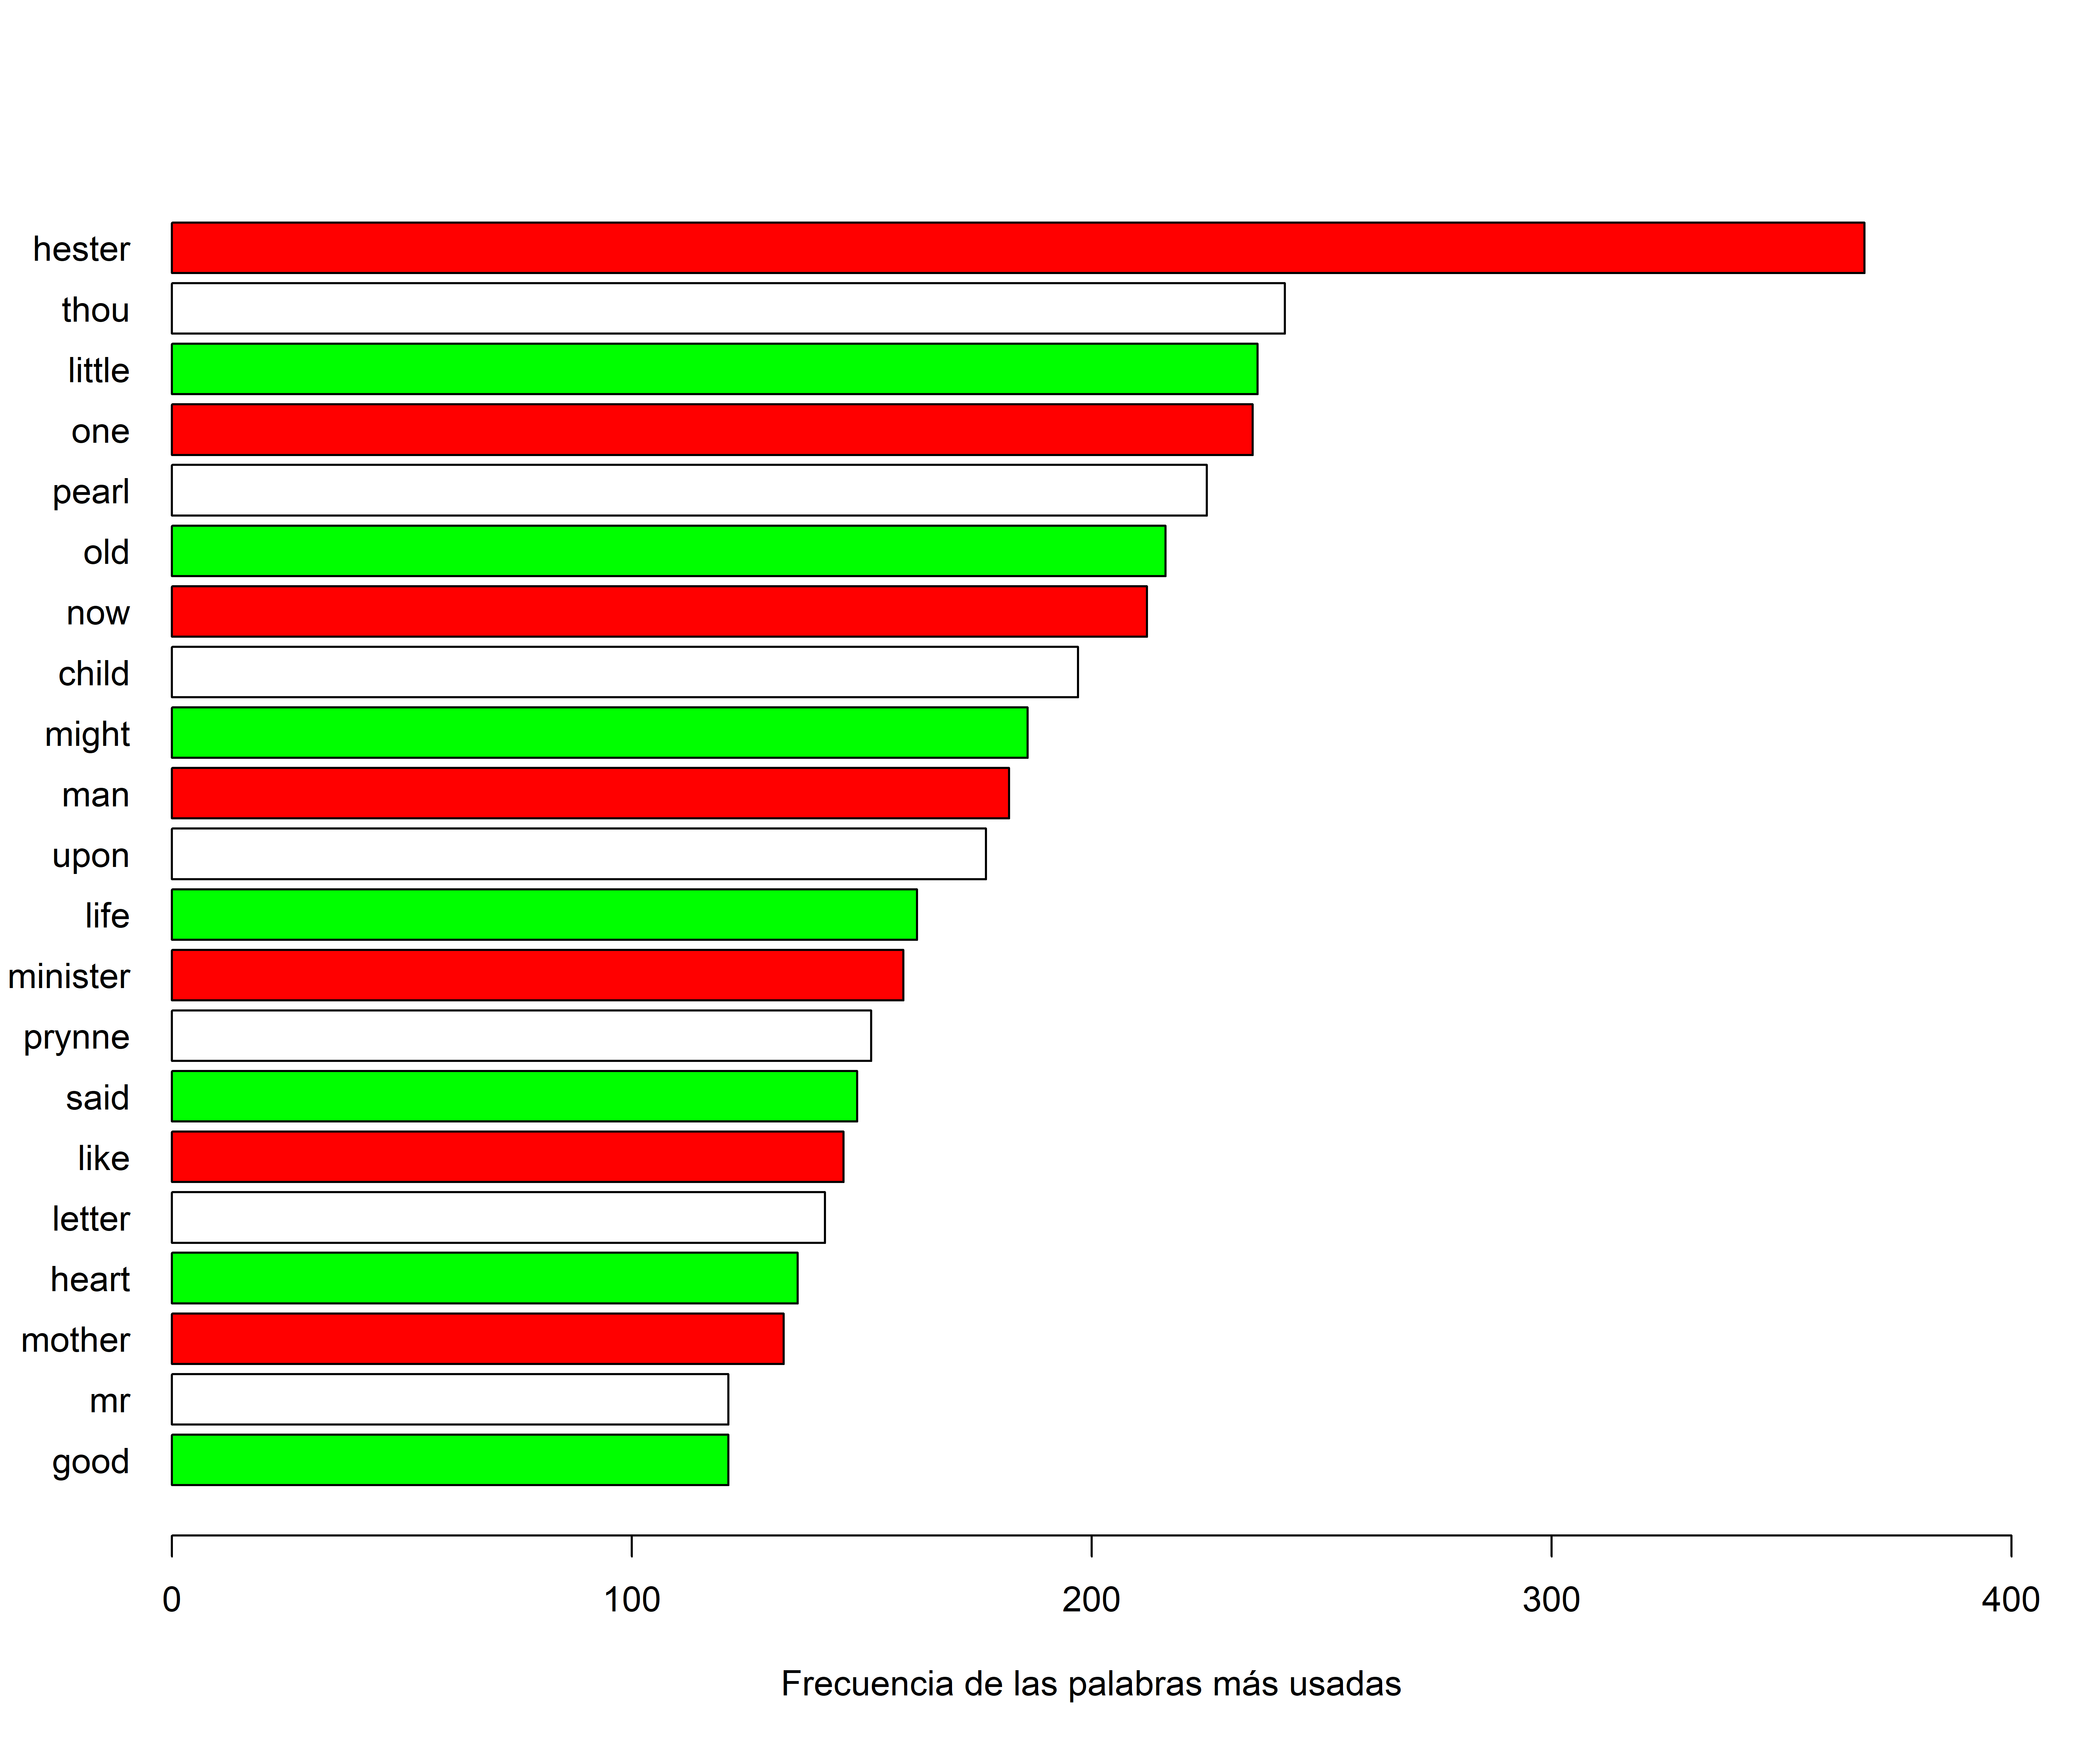
\includegraphics[scale=0.6]{Figures/palabrasFiltradasDecr.png}
\caption{Frecuencia decreciente de las palabras más usadas en el libro.}
\label{palabrasfiltradasdec}
\end{figure}

\begin{figure}
\centering
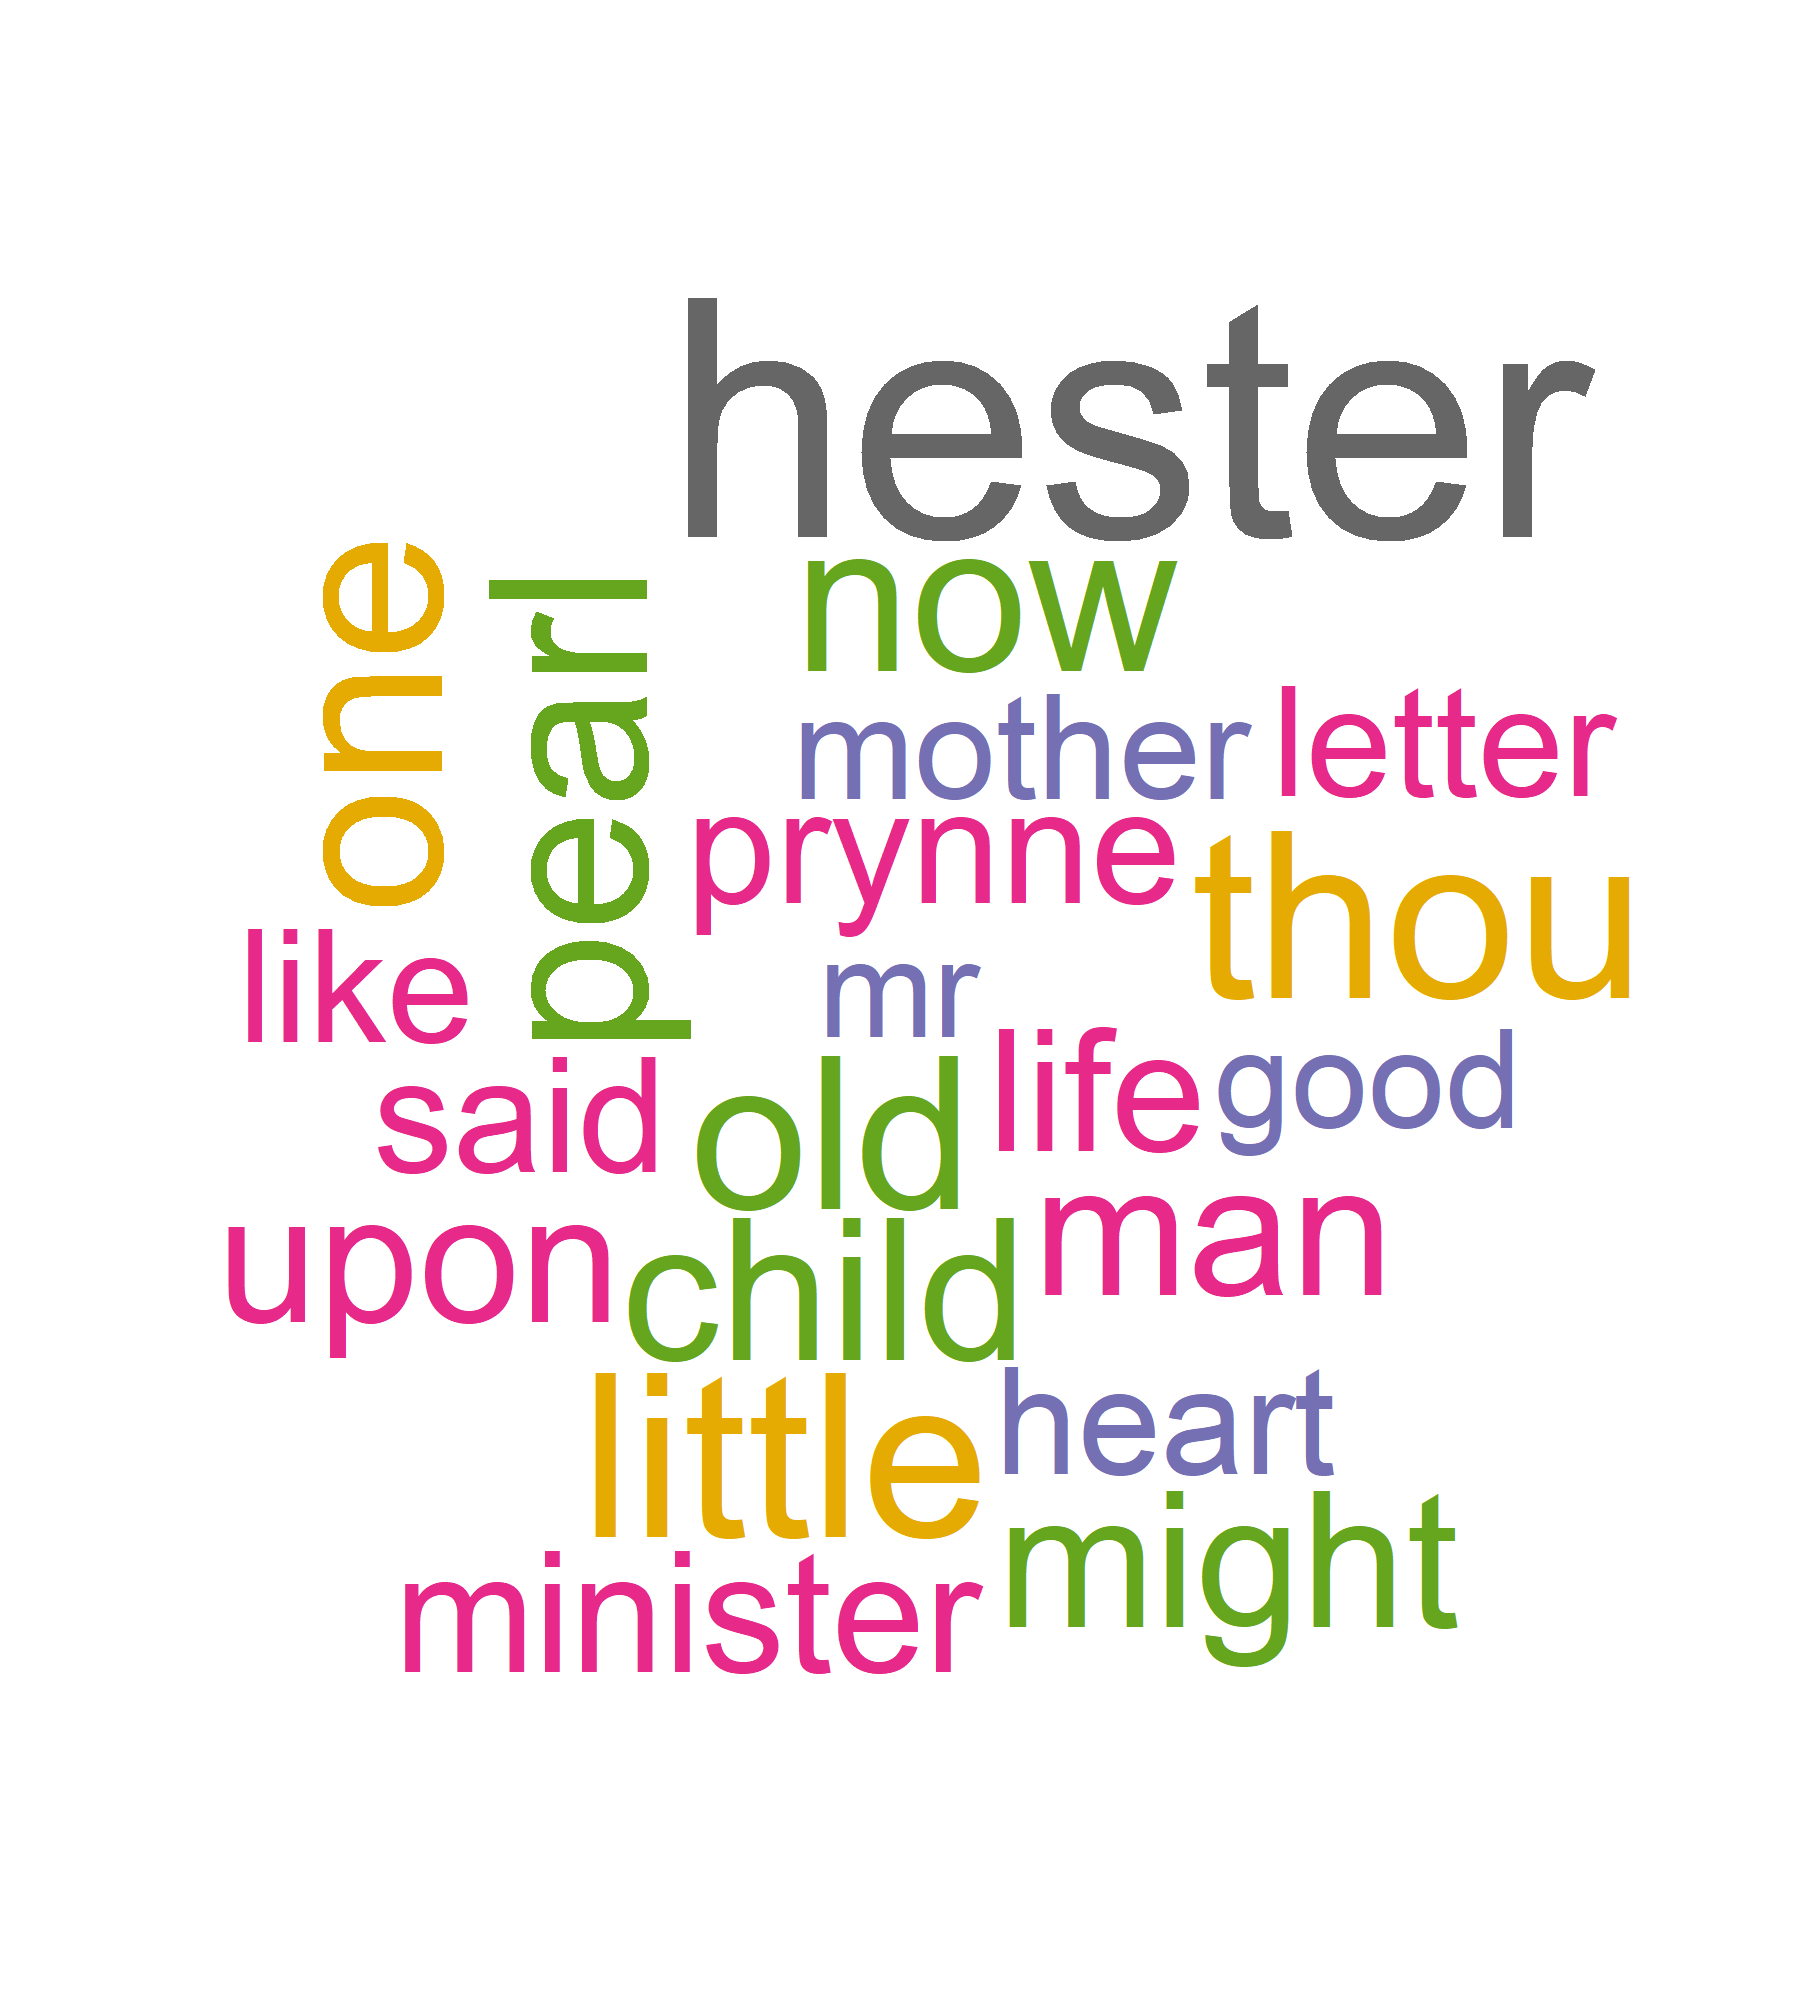
\includegraphics[scale=0.8]{Figures/wordcloud.png}
\caption{Nube de palabras más frecuentes en el libro}
\label{worldcloud}
\end{figure}


\bibliography{refProbabilidad}
\bibliographystyle{plain}

\end{document}